% --------------------------------------------------------------
% This is all preamble stuff that you don't have to worry about.
% Head down to where it says "Start here"
% --------------------------------------------------------------

\documentclass[12pt]{article}

\usepackage[margin=1in]{geometry}
\usepackage{amsmath,amsthm,amssymb}
\usepackage{graphicx}
\usepackage{subcaption}
\usepackage{algorithmicx}
\usepackage{algorithm}
\usepackage{algpseudocode}
\usepackage[colorlinks,linkcolor=blue]{hyperref}
\usepackage[noabbrev]{cleveref}
\usepackage{courier}
\usepackage{listings}


\oddsidemargin 0in
\evensidemargin 0in
\textwidth 6.5in
\topmargin -0.5in
\textheight 9.0in

\newcommand{\ignore}[1]{}
\def\pp{\par\noindent}

\newcommand{\assignment}[4]{
\thispagestyle{plain}
\newpage
\setcounter{page}{1}
\noindent
\begin{center}
\framebox{ \vbox{ \hbox to 6.28in
{CIS 4190/5190: Applied Machine Learning \hfill #1}
\vspace{4mm}
\hbox to 6.28in
{\hspace{2.5in}\large\bf\mbox{Homework #2}}
\vspace{4mm}
\hbox to 6.28in
{{\it Handed Out: #3 \hfill Due: #4}}
}}
\end{center}
}

\makeatletter
\renewcommand{\fnum@algorithm}{\fname@algorithm}
\makeatother

\lstset{basicstyle=\footnotesize\ttfamily,breaklines=true}
\lstset{framextopmargin=50pt,frame=bottomline}


\begin{document}

\assignment{Spring 2023}{1}{January 11}{January 25}

% --------------------------------------------------------------
%                         Start here
% --------------------------------------------------------------


{\bf Name: }  Qihang Dai\\

{\bf PennKey:} ahgdyycc\\

{\bf PennID:} 10578812\\

Note: This document is a read-only file. To create an editable version click on Menu in the top left corner of your screen and choose the Copy Project option. 
\section{Multiple Choice \& Written Questions}

\begin{enumerate}
\item
\begin{enumerate}
\item A
\item B
\end{enumerate}

\item 
\begin{enumerate}
\item B
\item A
\end{enumerate}

\item
\begin{enumerate}
\item C 0.92
\item B
\end{enumerate}

\item
\begin{enumerate}
\item D
\item \[\begin{aligned}
  Var(X) ={}& E[(X - E[X])^2] \\
  ={}& E[X^2 - 2XE[X] + E[X]^2] \\
  ={}& E[X^2] - 2E[X]E[X] + E[X]^2 \\
  ={}& E[X^2] - E[X]^2 \\
  \end{aligned}\]
\end{enumerate}

\item
\begin{enumerate}
\item B
\item A
\item D
\end{enumerate}
\end{enumerate}

\section{Python Programming Questions}

% Complete questions in your iPython notebook and place all results here.

% TODO: add matplotlib plot (Q4) here
TODO : Please add the matplotlib plot for Q4 below
\begin{figure}
  \centering
  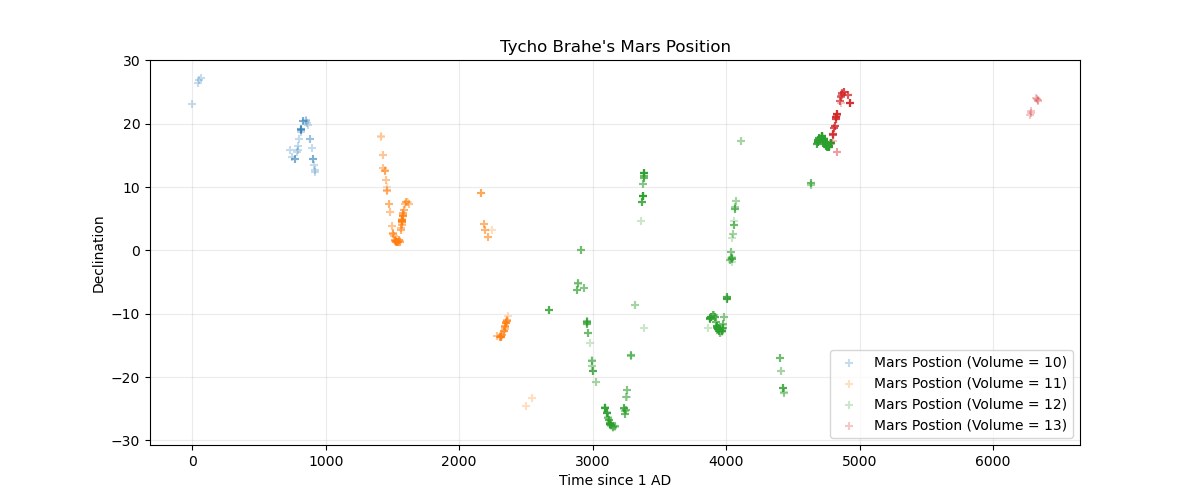
\includegraphics[width=0.8\textwidth]{example-figure.png}
  \caption{Figure for Q4 (MatplotLib)}
\end{figure}

\end{document} 